\subsection{DEFINITION OF A CONVEX FUNCTION}

DEFINITION 1. We say that a finite numerical function \(f\) , defined on an interval \(\mathrm{I} \subset \mathbf{R}\) , is convex on \(\mathrm{I}\) if, no matter what the points \(x, x'\) of \(\mathrm{I}\) , \((x < x')\) , every point \(\mathrm{M}_z\) of the graph \(\mathrm{G}\) of \(f\) such that \(x \leqslant z \leqslant x'\) lies below the segment \(\mathrm{M}_x\mathrm{M}_{x'}\) (or, what comes to the same, if every point of this segment lies above \(\mathrm{G}\) ) (fig.~2).

\pandocbounded{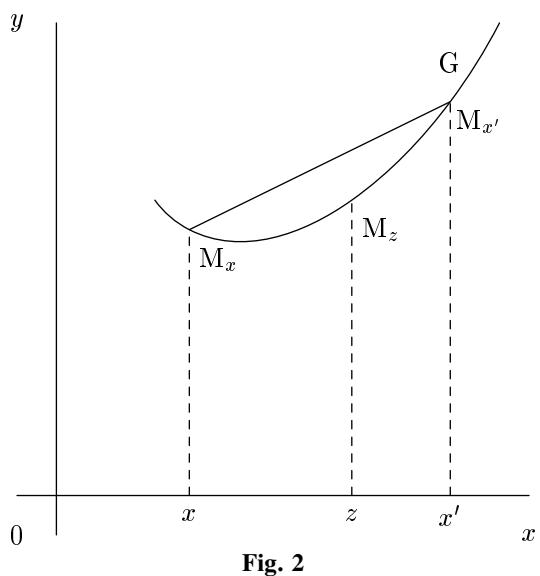
\includegraphics[keepaspectratio]{images/part001_0967d261.jpg}}

Taking account of the parametric representation of a segment (Gen.~Top., VI, p.~35), the condition for f to be convex on I is that one has the inequality

\[
f (\lambda x + (1 - \lambda) x ^ {\prime}) \leqslant \lambda f (x) + (1 - \lambda) f (x ^ {\prime})\tag{1}
\]

for each pair of points \((x, x')\) of I and every \(\lambda \in [0, 1]\) .

Definition 1 is equivalent to the following: the set of points in \(\mathbf{R}^2\) lying above the graph \(G\) of \(f\) is convex. Indeed, this condition is clearly sufficient for \(f\) to be convex on I; it is also necessary, for if \(f\) is convex on I, and if \((x,y)\) , \((x',y')\) are two points lying above \(G\) , then one has \(y \geqslant f(x)\) , \(y' \geqslant f(x')\) , from which, for \(0 \leqslant \lambda \leqslant 1\) ,

\[
\lambda y + (1 - \lambda) y ^ {\prime} \geqslant \lambda f (x) + (1 - \lambda) f \left(x ^ {\prime}\right) \geqslant f (\lambda x + (1 - \lambda) x ^ {\prime})
\]

by (1), which shows that every point of the segment with endpoints \((x, y)\) and \((x', y')\) lies above G.

Remark. On sees in the same way that the set of points lying strictly above G is convex. Conversely, if this set is convex one has

\[
\lambda y + (1 - \lambda) y ^ {\prime} > f (\lambda x + (1 - \lambda) x ^ {\prime})
\]

for \(0 \leqslant \lambda \leqslant 1\) and \(y > f(x)\) , \(y' > f(x')\) ; on letting \(y\) tend to \(f(x)\) and \(y'\) approach \(f(x')\) in this formula it follows that \(f\) is convex.

Examples. 1) Every (real) affine linear function \(ax + b\) is convex on \(\mathbf{R}\) .

\begin{enumerate}
\def\labelenumi{\arabic{enumi})}
\setcounter{enumi}{1}
\tightlist
\item
  The function \(x^{2}\) is convex on \(\mathbf{R}\) , since one has
\end{enumerate}

\[
\lambda x ^ {2} + (1 - \lambda) x ^ {\prime 2} - \left(\lambda x + (1 - \lambda) x ^ {\prime}\right) ^ {2} = \lambda (1 - \lambda) (x - x ^ {\prime}) ^ {2} \geqslant 0
\]

for \(0 \leqslant \lambda \leqslant 1\) .

\begin{enumerate}
\def\labelenumi{\arabic{enumi})}
\setcounter{enumi}{2}
\tightlist
\item
  The function \(|x|\) is convex on \(\mathbf{R}\) , since
\end{enumerate}

\[
\left| \lambda x + (1 - \lambda) x ^ {\prime} \right| \leqslant \lambda | x | + (1 - \lambda) \left| x ^ {\prime} \right|
\]

for \(0 \leqslant \lambda \leqslant 1\) .

It is clear that if \(f\) is convex on \(\mathbf{I}\) , then its restriction to any interval \(\mathbf{J} \subset \mathbf{I}\) is convex on \(\mathbf{J}\) .

Let \(f\) be a convex function on \(I\) , and \(x, x'\) two points of \(I\) such that \(x < x'\) ; if \(z \in I\) is exterior to \([x, x']\) then \(M_z\) lies above the line \(D\) joining \(M_x\) and \(M_{x'}\) ; this is an immediate consequence of the lemma.

One deduces from this that if z is a point such that \(x < z < x'\) and such that \(M_{z}\) lies on the segment \(M_{x}M_{x'}\) , then, for every other point \(z'\) such that \(x < z' < x'\) the point \(M_{z'}\) also lies on the segment \(M_{x}M_{x'}\) , for it follows from the above that \(M_{z'}\) is at the same time both above and below this segment; in other words, f is then equal to an affine linear function on \([x, x']\) .

DEFINITION 2. We say that a finite real function \(f\) defined on an interval \(\mathbf{I} \subset \mathbf{R}\) is strictly convex on \(\mathbf{I}\) if, for any points \(x, x'\) of \(\mathbf{I}\) ( \(x < x'\) ), every point \(\mathbf{M}_z\) of the graph \(\mathbf{G}\) of \(f\) such that \(x < z < x'\) lies strictly below the segment \(\mathbf{M}_x\mathbf{M}_{x'}\) (or, what comes to the same, if every point of the segment, apart from the endpoints, lies strictly above \(\mathbf{G}\) ).

In other words, we must have the inequality

\[
f (\lambda x + (1 - \lambda) x ^ {\prime}) <   \lambda f (x) + (1 - \lambda) f (x ^ {\prime})\tag{2}
\]

for every pair of distinct points \((x, x')\) of I and every \(\lambda\) such that \(0 < \lambda < 1\) .

The remarks that precede def. 2 show that for a convex function f to be strictly convex on I it is necessary and sufficient that there be no interval contained in I (not reducing to a single point) such that the restriction of f to this interval is affine linear.

Of the examples above, the first and third are not strictly convex; on the other hand, \(x^2\) is strictly convex on \(\mathbf{R}\) ; a similar calculation shows that \(1 / x\) is strictly convex on \(]0, +\infty[\) .

PROPOSITION 1. Let \(f\) be a finite real function, convex (resp. strictly convex) on an interval \(\mathbf{I} \subset \mathbf{R}\) . For every family \((x_i)_{1 \leqslant i \leqslant p}\) of \(p \geqslant 2\) distinct points of \(\mathbf{I}\) , and every family \((\lambda_i)_{1 \leqslant i \leqslant p}\) of \(p\) real numbers such that \(0 < \lambda_i < 1\) and \(\sum_{i=1}^{p} \lambda_i = 1\) , we have

\[
f \left(\sum_ {i = 1} ^ {p} \lambda_ {i} x _ {i}\right) \leqslant \sum_ {i = 1} ^ {p} \lambda_ {i} f (x _ {i})\tag{3}
\]

(resp.

\[
f \left(\sum_ {i = 1} ^ {p} \lambda_ {i} x _ {i}\right) <   \sum_ {i = 1} ^ {p} \lambda_ {i} f (x _ {i})).\tag{4}
\]

Since the proposition (for convex functions) reduces to the inequality (1) for \(p = 2\) we argue by induction for \(p > 2\) . The number \(\mu = \sum_{i=1}^{p-1} \lambda_i\) is \(> 0\) ; it is immediate that if \(a\) and \(b\) are the smallest and largest of the \(x_i\) then \(a \leqslant \sum_{i=1}^{p-1} \lambda_i x_i / \sum_{i=1}^{p-1} \lambda_i \leqslant b\) ; in other words, the point \(x = \frac{1}{\mu} \sum_{i=1}^{p-1} \lambda_i x_i\) belongs to I, and the induction hypothesis implies that \(\mu f(x) \leqslant \sum_{i=1}^{p-1} \lambda_i f(x_i)\) ; moreover we have, from (1), that

\[
f \left(\sum_ {i = 1} ^ {p} \lambda_ {i} x _ {i}\right) = f (\mu x + (1 - \mu) x _ {p}) \leqslant \mu f (x) + (1 - \mu) f (x _ {p}) \leqslant \sum_ {i = 1} ^ {p} \lambda_ {i} f (x _ {i}).
\]

One argues in the same way for strictly convex functions, starting from the inequality (2).

We say that a finite real function \(f\) is concave (resp. strictly concave) on I if \(-f\) is convex (resp. strictly convex) on I. It comes to the same to say that for every pair \((x, x')\) of distinct points of I and every \(\lambda\) such that \(0 < \lambda < 1\) one has

\[
f (\lambda x + (1 - \lambda) x ^ {\prime}) \geqslant \lambda f (x) + (1 - \lambda) f (x ^ {\prime})
\]

\[
(\text { resp. } f (\lambda x + (1 - \lambda) x ^ {\prime}) > \lambda f (x) + (1 - \lambda) f (x ^ {\prime})).
\]

